%! suppress = LineBreak
%! suppress = Unicode
%! suppress = MissingLabel
%! suppress = MissingImport
%! suppress = FileNotFound
\documentclass[../main.tex]{subfiles}

\begin{document}
    to procedury wywodzenia/wybierania przypadków testowych.

    \begin{table}[H]
        \begin{center}
            \begin{tabular}{p{8cm} p{8cm}}
                \begin{itemize}
                    \item systematyzują podejście do testowania
                    \item efektywne w znajdowaniu możliwych awarii
                    \item mogą uchronić przed redundantnymi testami
                \end{itemize}
                &
                \begin{itemize}
                    \item powtarzalne
                    \item oparte na modelach (np. działania oprogramowania)
                    \item dostarczają elementy pokrycia
                \end{itemize}
            \end{tabular}
        \end{center}
    \end{table}


    \begin{tabular}{|p{8cm}|p{8cm}|}
        \hline
        \textbf{Technika}              & \textbf{Element pokrycia}     \\
        \hline
        \hline
        Podział na klasy równoważności & Klasa równoważności           \\
        \hline
        Analiza wartości brzegowych    & Wartości brzegowe             \\
        \hline
        Drzewo klasyfikacji            & Liść / kombinacja liści       \\
        \hline
        Graf przyczynowo-skutkowy      & Kombinacja przyczyn           \\
        \hline
        Tablica decyzyjna              & Kombinacja warunków           \\
        \hline
        Testowanie maszyny stanowej    & Przejście / sekwencja przejść \\
        \hline
        Graf przepływu sterowania      & Ścieżka                       \\
        \hline
        CRUD                           & Cykl życia danej              \\
        \hline
    \end{tabular}

    \textbf{Hipoteza błędu} - każda technika projektowania testów zaprojektowana jest do
    wykrywania określonego typu awarii.

    \subsection{Techniki projektowania testów}

    \begin{table}[H]
        \begin{center}
            \begin{tabular}{ p{5cm} p{5cm} p{5cm} }
                \toprule
                \textbf{oparte na specyfikacji} & \textbf{oparte na strukturze} & \textbf{oparte na doświadczeniu} \\
                \toprule
                specyfikacja używa
                modeli, formalnych
                lub nieformalnych
                &
                testy tworzone na
                podstawie informacji
                o strukturze programu
                &
                testy tworzone na
                podstawie wiedzy,
                doświadczenia i
                intuicji testerów \\

                przypadki testowe
                mogą być tworzone
                systematycznie z
                tych modeli
                &
                można mierzyć
                stopień pokrycia
                oprogramowania i
                dodawać nowe testy
                by zwiększyć pokrycie
                &
                inne źródło informacji
                to wiedza o
                możliwych defektach i
                ich umiejscowieniu \\

                \begin{itemize}
                    \item klasy równoważności
                    \item wartości brzegowe
                    \item tablice decyzyjne
                    \item grafy P-S
                    \item maszyna stanowa
                    \item drzewa klasyfikacji
                    \item przypadki użycia
                    \item testowanie losowe
                \end{itemize}
                &
                \begin{itemize}
                    \item pokrycie instrukcji
                    \item pokrycie decyzji
                    \item pokrycie warunków
                    \item pokrycie MC/DC
                    \item pokrycie przepływu danych
                    \item pokrycie pętli
                    \item pokrycie ścieżek
                    \item testowanie mutacyjne
                \end{itemize}
                &
                \begin{itemize}
                    \item t. eksploracyjne
                    \item zgadywanie błędów
                    \item ataki usterkowe
                    \item t. z listą kontrolną
                    \item testowanie ad hoc
                \end{itemize} \\
            \end{tabular}
        \end{center}
    \end{table}


    \begin{table}[H]
        \begin{center}
            \begin{tabular}{| p{8cm} p{8cm}|}
                \hline
                \multicolumn{2}{|c|}{ \textbf{Analiza wartości brzegowych}} \\
                \hline
                \begin{itemize}
                    \item technika oparta na podziale na klasy równoważności
                    \item działa dla klas, na których zadany jest porządek liniowy
                \end{itemize} &
                \begin{itemize}
                    \item wartość brzegowa = wartość min/max zadanej klasy równoważności
                    \item można rozważać wartości brzegowe dla wejścia i wyjścia
                \end{itemize}
                \\
                \hline
                \hline
                \multicolumn{2}{|c|}{ \textbf{Tablice decyzyjne}} \\
                \hline
                \textbf{Tablice decyzyjne}
                \begin{itemize}
                    \item testowanie kombinacji warunków
                    \item dobra metoda do testowania logiki biznesowej
                    \item pozwala na systematyczne sprawdzanie wszystkich kombinacji
                    \item ułatwia wykrywanie
                    \begin{itemize}
                        \item brakującej specyfikacji
                        \item błędnej (sprzecznej) specyfikacji
                    \end{itemize}
                \end{itemize}
                &
                \textbf{Minimalizacja tablicy} - jeśli wszystkie kombinacje pewnych warunków dają te same akcje, możemy je scalić. \\
                \hline
                \hline
                \multicolumn{2}{|c|}{ \textbf{Grafy przyczynowo-skutkowe}} \\
                \hline
                \begin{itemize}
                    \item stosowane w tych samych sytuacjach co tablice decyzyjne
                    \item graficzna reprezentacja zależności między przyczynami a skutkami
                    \item prosta transformacja na tablice decyzyjne
                \end{itemize}
                &
                \raisebox{-\totalheight}{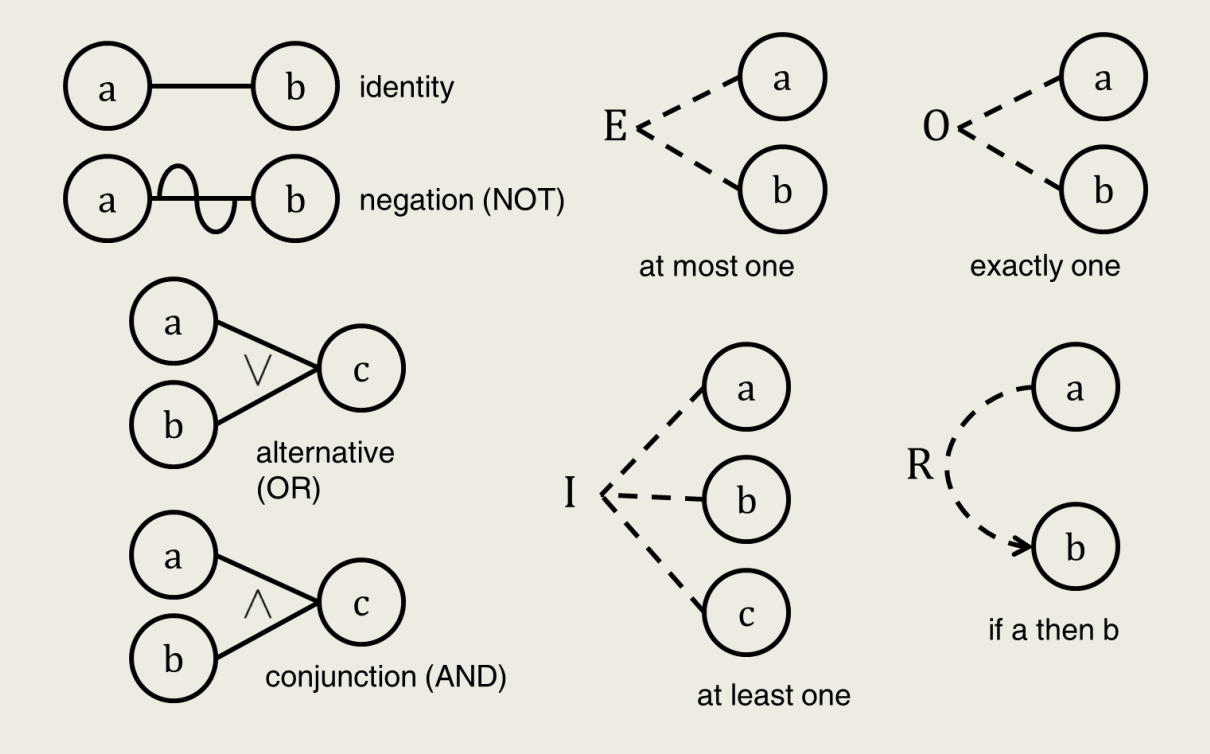
\includegraphics[width=8cm]{graf.png}} \\
                \hline
            \end{tabular}
        \end{center}
    \end{table}


\end{document}